% !TeX encoding = UTF-8
\documentclass[twocolumn]{jarticle}
%\documentclass[uplatex]{jsarticle}
%-------------------------------------------------------------------------%
\newcommand{\ctext}[1]{\raise0.2ex\hbox{\textcircled{\scriptsize{#1}}}}
\newcommand{\red}[1]{\textcolor{red}{#1}}
\usepackage{abst}                   % abst.styの呼び出し
\usepackage{color}
\usepackage[super]{cite}            % 文献参照の設定変更パッケージ
\usepackage[dvipdfmx]{graphicx}
\usepackage{here}                   % here.styの呼び出し
\usepackage{amsmath,amssymb}
\usepackage{ascmac}
\usepackage{url}
\usepackage{comment}
\usepackage{siunitx}
\renewcommand\citeform[1]{#1)}      % 文献参照を^(1))にする
\begin{document}
%-------------------------------------------------------------------------%
% 表紙
%\thispagestyle{empty}
%\include{cover.tex}
%\newpage

%-------------------------------------------------------------------------%
% ページ番号の設定
%\setcounter{page}{1}
%\pagenumbering{roman}

% 目次
%\tableofcontents4
%\newpage

% •表目次
%\listoftables

% 図目次
%\listoffigures

%-------------------------------------------------------------------------%
% title
\twocolumn[
    \centering
    \fontsize{11pt}{0pt}\selectfont
    {\gt エアシリンダ型人工筋肉の開発}
    \vspace{4.5pt}

    \fontsize{9pt}{0pt}\selectfont
    {\rm Development of air cylinder type artificial muscle}
    \vspace{1zw}

    \raggedright
    \fontsize{9pt}{0pt}\selectfont
    \hspace{8zw}
    発表者  三宅 悠暉
    \hspace{11.2zw}%{5.6zw}
    主任教員  平光 立拓 助教

    \vspace{0.5zw}
    \hspace{29.6zw}%{5.6zw}
    指導教員  関 啓明 教授, 辻 徳生 准教授
    \vspace{3zw}
]

% main
\fontsize{9pt}{0pt}\selectfont
\setlength{\baselineskip}{12pt}
\section{緒言}%===========================
エアシリンダは生産現場などに多く使われている.
しかし,長いストロークを持ちつつも,コンパクトに使用するような場合には適合しない.
よって,十分にストロークがありつつも,設置しやすい直動アクチュエータが求められている.
そこで,曲げられるエアシリンダを提案する.
本研究では曲げられるエアシリンダを``エアシリンダ型人工筋肉''と呼ぶ.
エアシリンダ型人工筋肉は柔らかい素材で構成されている.
そのため,曲がった状態で配置・動作し,高ストロークを有しつつもコンパクトに設置することができる.
しかし,エアシリンダ型人工筋肉は曲がった状態において,チューブと紐が接触する現象が起こる.
この接触がエアシリンダ型人工筋肉の出力にどのような影響があるか確認する必要がある.
\par
本研究は4つの段階から構成される.
1つ目にエアシリンダ型人工筋肉の開発を行う.
2つ目に開発したエアシリンダ型人工筋肉の基礎特性の測定を行う.
3つ目に,曲がったエアシリンダ型人工筋肉の理論出力を基礎特性を使用して導出し,実験値と比較する.
これらの結果よりチューブと紐の接触がエアシリンダ型人工筋肉の出力にどのくらい影響するか確認を行う.
4つ目にエアシリンダ型人工筋肉を用いた機構の開発を行う.
エアシリンダ型人工筋肉を機構に応用することにより制御性について評価を行う.
これらの内容を踏まえて,エアシリンダ型人工筋肉が曲げた状態で配置及び動作可能であるか評価を行う.

% 1.エアシリンダ型人工筋肉の開発
% 2.基礎特性の測定
% 3.曲がったエアシリンダ型人工筋肉の出力の理論化と実験値の比較
% 4.揺動アームの制御
\begin{figure}[t]
  \centering
  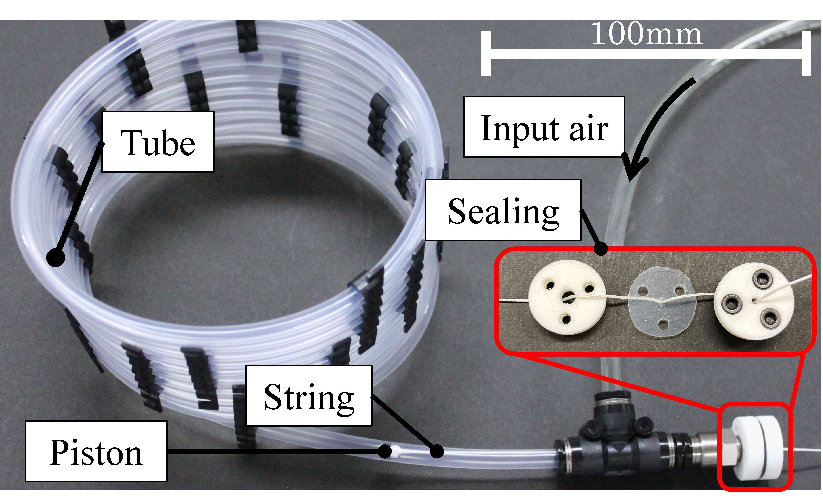
\includegraphics[width=85mm]{_pdf/細径柔軟エアシリンダ-1本.pdf}
  \caption{Air cylinder type artificial muscle}
  \label{Air cylinder type artificial muscle}
\end{figure}

\section{エアシリンダ型人工筋肉の開発}%-----------
開発したエアシリンダ型人工筋肉とシール内部構造を図\ref{Air cylinder type artificial muscle}に示す.
エアシリンダ型人工筋肉は4つの部品から構成される.
それらはチューブ,紐,ピストン,シール部である.
チューブは曲げやすさ,ピストンとの摩擦係数の小ささを重視し,フッ素樹脂チューブ(ニチアス株式会社,材質:ナフロン\textregistered,内外径:$\SI{5}{mm}$, $\SI{6}{mm}$,最小曲げ半径:$\SI{35}{mm}$)を選択した.
紐はシール部との摩擦係数の小ささ,高強度,高剛性を重視し,高強度化学繊維ロープ(ハヤミ工産株式会社,材質:イザナス®,線形:$\SI{0.60}{mm}$,破断強度:$\SI{360}{N}$,破断伸度:$\SI{5.5}{N}$)を選択した.
ピストンはチューブとの摩擦係数の小ささ,曲がったチューブ内壁からのエア漏れ防止を重視し,2枚のフッ素ゴムリング(株式会社廣杉計器,材質:フッ素ゴム,内外径:$\SI{3.0}{mm}$, $\SI{5.0}{mm}$,厚み:$\SI{1.0}{mm}$,硬度:\SI{80}{\degree}(デュロメータA))を2枚のPLA樹脂部品で挟み込む構造とした.
シール部は耐候性を重視し,シリコンゴムシート(材質:シリコン,厚さ:1 mm,硬度:\SI{70}{\degree}(デュロメータA))を選択した.
なお,ゴムシートに穴をあけて紐を通している.
紐を通したゴムシートを2つのプラスチック部品を3本のボルトにより挟み込む.

\section{基礎特性の測定}%-----------
エアシリンダ型人工筋肉の各部品間には抵抗力が存在する.
1つ目は,シール部と紐の接触による摩擦抵抗$D_s$である.
2つ目は,チューブとピストンの接触による摩擦抵抗$D_\mathrm{p}$である.
3つ目は,チューブと紐の接触による摩擦抵抗$D_\mathrm{t}$である.
抵抗$D_\mathrm{s}$,$D_\mathrm{p}$は印加圧力によって変化すると考えられる.
抵抗$D_\mathrm{t}$はチューブと紐の接触角$\theta$によって変化すると考えられる.
これら3つの抵抗力$D_\mathrm{s}(P_\mathrm{in})$,$D_\mathrm{p}(P_\mathrm{in})$,$D_\mathrm{t}(\theta)$を実験により測定した.
以下に各抵抗$D_\mathrm{s}(P_\mathrm{in})$,$D_\mathrm{p}(P_\mathrm{in})$,$D_\mathrm{t}(\theta)$の実験式を示す.
\begin{align}
  D_\mathrm{s} & = \num{-4.0e-4}P_\mathrm{in} + \num{5.6e-4} \label{eq:D_s} \\
  D_\mathrm{p} & = \num{2.1e-3}P_\mathrm{in} + \num{4.0e-4}  \label{eq:D_p} \\
  D_\mathrm{t} & = 0.981e^{0.090\theta}\label{eq:D_t}
\end{align}
なお,式\eqref{eq:D_t}とキャプスタン方程式よりチューブと紐の摩擦係数$\mu$は0.090ということが求められる.

\section{環状に曲がったエアシリンダ型人工筋肉の理論出力}%-----------
\subsection{理論出力の導出}%-----------
エアシリンダ型人工筋肉のモデルを図\ref{Model of artifucialmuscle}に示す.
エアシリンダ型人工筋肉は曲率半径$r$で環状に曲がった状態であり,ピストンは巻き角$\theta$の位置にある.
巻き角$\theta$,印加圧力$P_\mathrm{in}$における人工筋肉の出力は$F$とする.
なお,エアシリンダ型人工筋肉の紐直径を$d_\mathrm{string}$,チューブ内径(ピストン直径)は$d_\mathrm{tube}$である.また,シール部と紐の抵抗力は$D_\mathrm{s}$,チューブとピストンの抵抗力は$D_\mathrm{p}$である.
モデルにおいては,チューブと紐が接触する角度を巻き角$\theta$と仮定する.
これらの条件化におけるチューブと紐が接触している状態のエアシリンダ型人工筋肉の理論出力$F_\mathrm{th}$を導出した結果を式\eqref{F}に示す.
\begin{figure}[t]
  \centering
  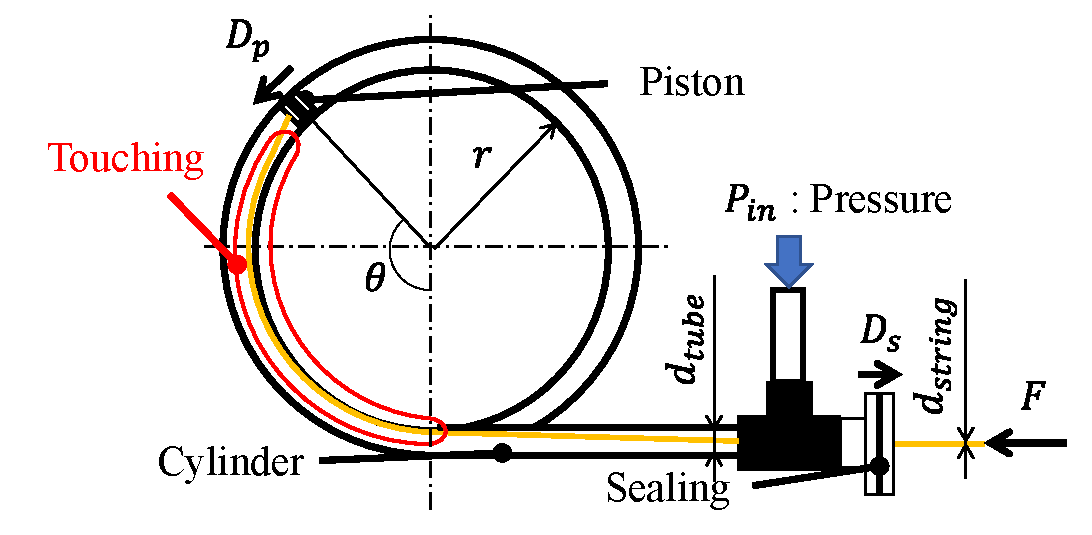
\includegraphics[width=85mm]{_pdf/model_artifucialmuscle.pdf}
  \caption{Model of artifucialmuscle}
  \label{Model of artifucialmuscle}
\end{figure}

\begin{equation}
  \label{F}
  F_\mathrm{th}=\frac{1}{e^{\mu\theta}} (\frac{π}{4}d_\mathrm{tube}^2 P_\mathrm{in}-D_\mathrm{p} )-D_\mathrm{s}
\end{equation}

\subsection{理論値と実験値の比較}%-----------
エアシリンダ型人工筋肉が半径$r$で環状に曲がった状態のチューブ位置(巻き角)$\theta$における出力$F$を計測する.
紐の先端をフォースゲージに接続し,人工筋肉に圧力$P_\mathrm{in}$を印加し,出力$F$を測定する.
なお,フォースゲージ及び紐の先端を速度$v=\SI{5}{mm/s}$で直動させる.
チューブの巻き半径$r$は$\SI{100}{mm}$と$\SI{150}{mm}$の2パターンである.
印加圧力$P_\mathrm{in}$は$\SI{100}{kPa} \sim \SI{400}{kPa}$の範囲において$\SI{100}{kPa}$刻みでそれぞれ5回測定を行う.測定終了の判定は,出力$F$が5秒間$\SI{0}{N}$となる場合である.
\par
チューブの巻き半径$r=\SI{100}{mm}$,$\SI{150}{mm}$の理論値(破線)と実験値(実線)をそれぞれ図\ref{r=100mm},図\ref{r=150mm}に示す.また,実験値には$\SI{0.1}{Hz}$のローパスフィルタを実施した.図\ref{r=100mm},\ref{r=150mm}より,概ね理論値と実験値の傾向が一致していることがわかる.しかし,図\ref{r=100mm},図\ref{r=150mm}の実験値を比較すると,各印加圧力$P_\mathrm{in}$によって傾きが異なることがわかる.この原因は,ピストン抵抗力$D_\mathrm{p}$がチューブの曲げ半径$r$によって異なるためである.よって,エアシリンダ型人工筋肉が曲がった状態においては,チューブの曲げ半径$r$とピストン抵抗$D_\mathrm{p}$の関係を明らかにする必要がある.
\begin{figure}[t]
  \centering
  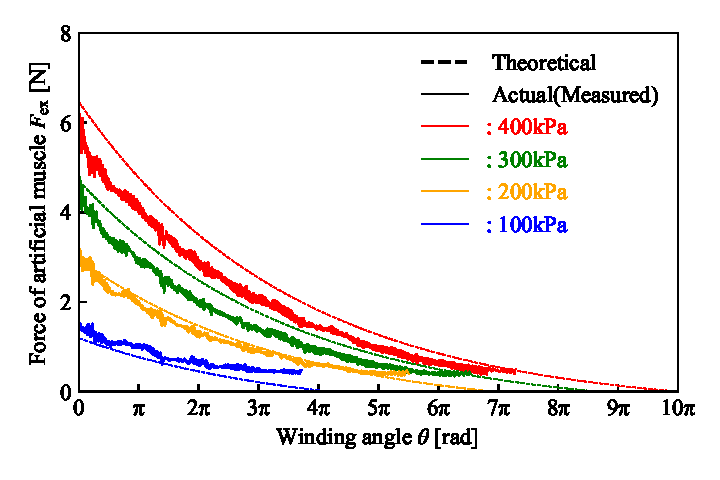
\includegraphics[width=85mm]{_pdf/result_100mm.pdf}
  \caption{Result of winding radius $r=100$}
  \label{r=100mm}
\end{figure}

\begin{figure}[t]
  \centering
  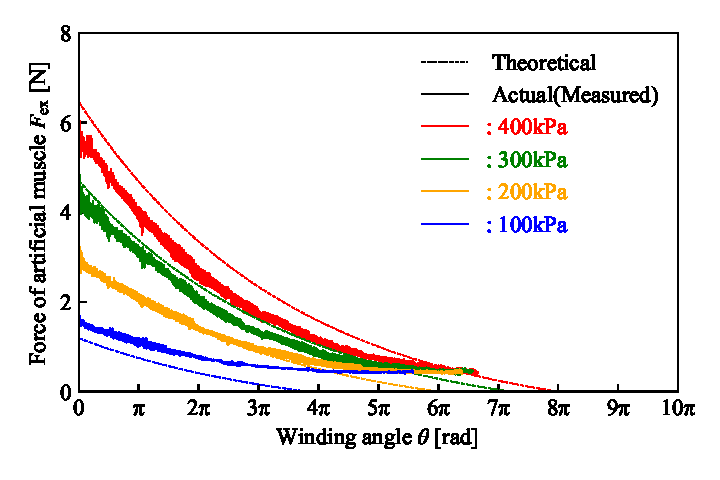
\includegraphics[width=85mm]{_pdf/result_150mm.pdf}
  \caption{Result of winding radius $r=150$}
  \label{r=150mm}
\end{figure}

\section{エアシリンダ型人工筋肉を用いた揺動アームの開発}%-----------
\subsection{揺動アームの構造}
エアシリンダ型人工筋肉を機械要素として応用する方法を検討する.
機械要素として応用する場合には,エアシリンダ型人工筋肉の本数や配置を設計および制御方法について検討する必要がある.
そこで,エアシリンダ型人工筋肉を揺動アームに4本取り付け,アームの角度を制御する.
図\ref{Swing arm}に揺動アームの概要を示す.
エアシリンダ型人工筋肉はアームに対し対抗配置(2本×2セット)する.
なお,エアシリンダ型人工筋肉の印加圧力は2系統であり,それぞれ圧力$P_\mathrm{a}$,$P_\mathrm{b}$とする.
また,揺動アーム根本に取り付けたプーリによりエアシリンダ型人工筋肉の直動運動を回転運動に変換する.
アームの揺動角度を$\theta$とし,アームに取り付けた3軸ジャイロ+3軸加速度センサにより角度$\theta$を計測する.
\begin{figure}[t]
  \centering
  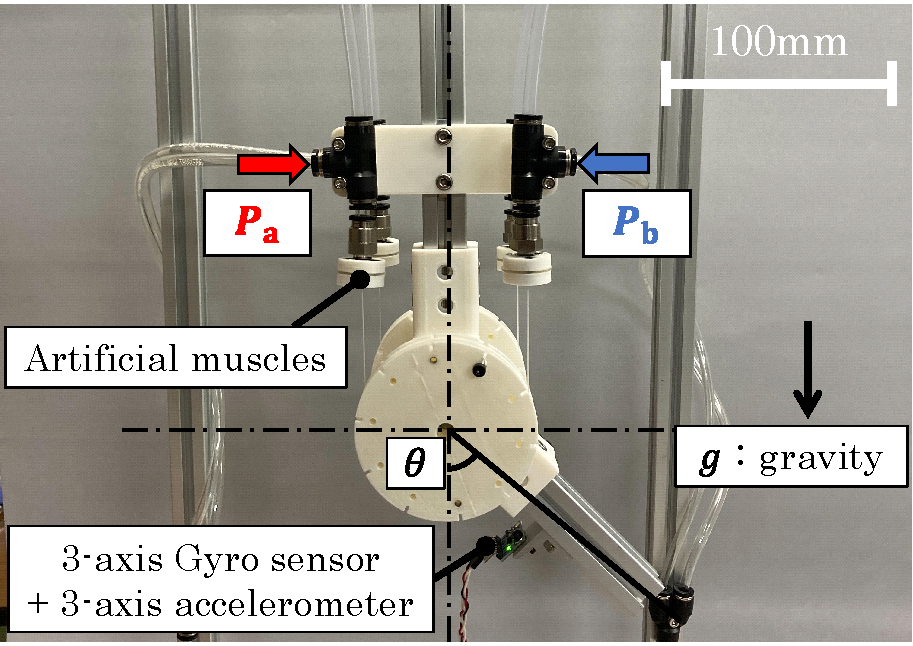
\includegraphics[width=80mm]{_pdf/swing_arm.pdf}
  \caption{Swing arm}
  \label{Swing arm}
\end{figure}

\subsection{揺動アームの角度制御}
目標値を揺動アームの角度$\phi$とした場合の,制御性について評価を行う.
制御方法は2系統の印加圧力の平均$P_\mathrm{ave}=(P_\mathrm{a} + P_\mathrm{b})/2$を一定値$P_\mathrm{ave}=\SI{220}{kPa}$として入力し,差圧$\Delta P = P_\mathrm{a} - P_\mathrm{b}$を制御値とする.
目標値は$\phi_\mathrm{p} = 90 \sin(0.01t)$とし,実角度$\phi$を測定する.
なお,エアシリンダ型人工筋肉のチューブは真っすぐな状態で測定を行った.
\par
図\ref{Frequency response}に測定結果を示す.
青色のプロットが実角度$\phi$,オレンジ色のプロットが目標値$\phi_\mathrm{p}$,灰色のプロットが目標値$\phi_\mathrm{p}$と実角度$\phi$の差である.
図\ref{Frequency response}より,概ね目標値$\phi_\mathrm{p}$に対して実角度$\phi$が概ね追従していることがわかる.
また,目標値$\phi_\mathrm{p}$が$\SI{90}{\degree}$と$\SI{-90}{\degree}$に向かうときでは実角度$\phi$の追従性が異なることがわかる.
これは,エアシリンダ型人工筋肉1本1本の特性がわずかに異なり,追従性に影響を及ぼしたと考えられる.
これらの結果より,エアシリンダ型人工筋肉を揺動アームに応用しアームの角度制御をする時,概ね制御できることがわかった.
ただし,エアシリンダ型人工筋肉の特性が1本1本異なることを考慮して機構に応用する必要があることが明らかとなった.
\begin{figure}[t]
  \centering
  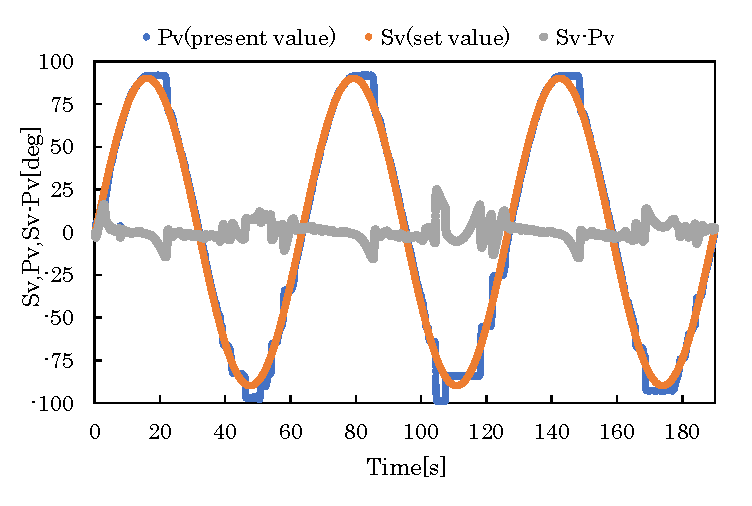
\includegraphics[width=85mm]{_pdf/result_frequency_response.pdf}
  \caption{Frequency response}
  \label{Frequency response}
\end{figure}

\section{結言}%-----------
%わかったことをより詳細に述べる
曲がった状態で配置・動作し,高ストロークを有しつつもコンパクトに設置することができるエアシリンダ型人工筋肉を開発した.
開発したエアシリンダ型人工筋肉の各部品間における抵抗力を測定し,エアシリンダ型人工筋肉が動作する上で問題ないか確認した.
2つの抵抗$D_\mathrm{s}$,$D_\mathrm{p}$と摩擦係数$\mu$は小さいことがわかり,エアシリンダ型人工筋肉の各部品選定及び構造は妥当であることがわかった.
次に,曲がったエアシリンダ型人工筋肉の理論出力$F_\mathrm{th}$を導出した.
理論出力$F_\mathrm{th}$は巻付け角度$\theta$の増加に伴って指数関数的に減少することが明らかとなった.
さらに,実験値と比較した結果,概ね理論値と実験値が一致した.
ただし,チューブの曲げ半径$r$によって実験値がわずかに異なることがわかった.
これらの結果より,チューブの曲げ半径$r$とピストン抵抗$D_\mathrm{p}$の関係を明らかにする必要がある.
最後に,エアシリンダ型人工筋肉を揺動アームに応用し,アームの角度制御性について評価を行った.
目標値$\phi_\mathrm{p}$に対して実角度$\phi$が概ね一致し,角度制御性も良好であることがわかった.
これらの内容を踏まえて,エアシリンダ型人工筋肉が曲げた状態で配置及び動作が可能であることを示した.
%refarence
\bibliographystyle{junsrt}
\bibliography{ref}

\end{document}
